
\documentclass[12pt]{article}

\usepackage[margin=2cm]{geometry}

\usepackage[utf8]{inputenc}
\usepackage[T1]{fontenc}



%% Loading tcolorbox for easy laying out of
%% LaTeX code and output side-by-side
\usepackage{xcolor}
\usepackage{tcolorbox}
\tcbuselibrary{minted}
\newtcblisting{mybox}{colback=white,minted language=latex,listing side text,righthand width=.2\textwidth}

\usepackage{tikzducks}
\usepackage{tikz}
\usetikzlibrary {shapes.callouts}


\begin{document}


\begin{enumerate}
    \item Tara duck\\
        \begin{tikzpicture}
            \duck[longhair]
            \node[inner sep=0pt] (russell) at (0,0)
            {
\includegraphics[width=.1\textwidth]{laptop.png}};
        \end{tikzpicture}
    \item Produckt manager \\
        
\begin{tikzpicture}
            \duck[tshirt,
            jacket=gray,
            tie,
            squareglasses=blue!50!black]
        \end{tikzpicture}
    \item duck[ ] myDucksInARow = \{duck1, duck2, duck3\};\\
        $\Biggr[
        
\begin{tikzpicture}[x=5mm,y=5mm,baseline={([yshift=-.5ex]current bounding box.center)}]
            \duck[signpost=0]
        \end{tikzpicture} ,
        
\begin{tikzpicture}[x=5mm,y=5mm,baseline={([yshift=-.5ex]current bounding box.center)}]
            \duck[signpost=1] 
        \end{tikzpicture} ,
        
\begin{tikzpicture} [x=5mm,y=5mm,baseline={([yshift=-.5ex]current bounding box.center)}]
            \duck[signpost=2]
        \end{tikzpicture}
       \Biggr]\\$
    \item Philospher duck\\
       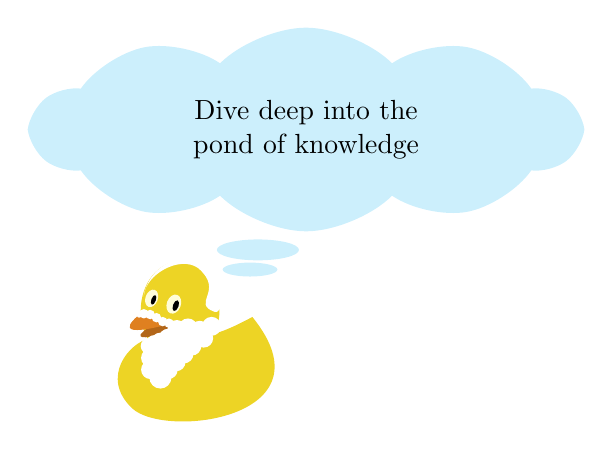
\begin{tikzpicture}
            \duck[laughing,
                recedinghair=white,beard]
                \node[cloud callout, inner sep= 0pt, fill=cyan!20, aspect=4,  cloud puff arc=90, text width=5cm, text centered, xshift=2cm, yshift=2.5cm, callout relative pointer={(-.2,-.5)}] at (bill) {Dive deep into the \\pond of knowledge};
        \end{tikzpicture}

\end{enumerate}

\end{document}
